\ifx\boi\undefined\ifx\problemname\undefined
\providecommand\sampleinputname{}
\providecommand\sampleoutputname{}
\documentclass[german]{templates/boi}
\problemlanguage{.de}
\fi
\newcommand{\boi}{Baltische Informatikolympiade}
\newcommand{\practicesession}{Practice Session}
\newcommand{\contestdates}{27. April - 1. Mai, 2018}
\newcommand{\dayone}{Tag 1}
\newcommand{\daytwo}{Tag 2}
\newcommand{\licensingtext}{Diese Aufgabenstellung ist unter der CC BY-SA 4.0 lizensiert.}
\newcommand{\problem}{Aufgabe}
\newcommand{\inputsection}{Eingabe}
\newcommand{\outputsection}{Ausgabe}
\newcommand{\interactivity}{Interaktivität}
\newcommand{\grading}{Grading}
\newcommand{\scoring}{Scoring}
\newcommand{\constraints}{Beschränkungen}
\renewcommand{\sampleinputname}{Beispieleingabe}
\renewcommand{\sampleoutputname}{Beispielausgabe}
\newcommand{\sampleexplanation}[1]{Beschreibung zu Beispiel #1}
\newcommand{\sampleexplanations}{Beschreibung der Beispiele}
\newcommand{\timelimit}{Zeitlimit}
\newcommand{\memorylimit}{Speicherlimit}
\newcommand{\seconds}{s}
\newcommand{\megabytes}{MB}
\newcommand{\group}{Gruppe}
\newcommand{\points}{Punkte}
\newcommand{\limitsname}{Limits}
\newcommand{\additionalconstraints}{Zusätzliche Beschränkungen}
\newcommand{\testgroups}{
Deine Lösung wird auf mehreren Testgruppen ausgeführt werden, von denen jede eine bestimmte Punktzahl wert ist.
Jede Testgruppe enthält mehrere Testcases. Um Punkte für eine Testgruppe zu bekommen, müssen alle Testfälle in der entsprechenden Gruppe gelöst werden.
Deine finale Punktzahl wird die maximal erreichte Punktzahl in allen Einsendungen sein.
}
\fi
\def\version{jury-1}
\problemname{Alternating Current}

Fredrik ist zu Hause und spielt mit seiner selbstgebauten Eisenbahn, auf die er sehr stolz ist. Die Eisenbahn besteht aus $N$ im Kreis angeordneten Schienen, die von $1$ bis $N$ im Uhrzeigersinn durchnummeriert sind. Der Zug erhält seinen Strom von $M$ an dem Kreis angebrachten Drähten. An jeder Schiene läuft mindestens eine solchen Draht entlang.

%Fredrik is at home, playing with a custom-built model railway which he is very proud of.
%The railway consists of $N$ segments connected in a circle, numbered $1, 2, \dots, N$ in clockwise order.
%Electricity to the train is provided through $M$ curved wires that pass along the circle. Each segment has at least one wire that goes along it.


Leider wird Fredrik recht langweilig mit seiner Eisenbahn, die nur im Kreis fährt, woraufhin er entscheidet, eine \emph{Weiche} zu jeder Schiene hinzuzufügen, um Zugentgleisungen und andere aufregende Szenarios zu verursachen. Aber die Weichen brauchen ebenfalls Elektrizität. Und zwar nicht irgendeinen Strom; Sie brauchen \emph{Wechselstrom}. \footnote{Das macht Sinn, denn die Eisenbahn ist eine schwedische -- in Schweden verwenden alle Weichen (``växlar'') Wechselstrom (``växelström'').}

%However, Fredrik is becoming bored with his circling train and decides to add a \emph{train switch} to every segment, which he could use to cause derailing accidents and other exciting scenarios. But the switches also need electricity.
%And not just any kind of electricity; they specifically need \emph{alternating current}.\footnote{This makes sense because the railway is a Swedish one -- in Sweden, all train switches (``växlar'') use alternating current (``växelström'').}
% Sorry about the terrible pun. If it translates into your language you can remove the footnote.


Um Wechselstrom zu bekommen, wird Strom benötigt, der in beide Richtungen fließt.
Jeder Draht kann nur Strom in eine Richtung (entweder im Uhrzeigersinn oder gegen den Uhrzeigersinn) liefern, aber Fredrik darf entscheiden, in welche.
Er muss also eine Entscheidung für die Stromrichtung jedes Drahtes treffen, um zu erreichen, dass jede Weiche mindestens mit je einem Draht für jede Stromrichtung verbunden ist.

Kannst du Fredrik hierbei helfen?

%The way you get alternating current, Fredrik figures, is by having current
%that goes in both directions. Each wire only gives current in one direction
%(either clockwise or counter-clockwise) but Fredrik is free to decide which.
%Thus, what he wants to do is to make a decision about the direction of the current in each wire,
%so that every track segment is covered by both a wire with clockwise-directed current and a wire with 
%counter-clockwise-directed current.

%Can you help Fredrik with this task?

\vspace{2mm}
%\hspace*{2mm}
\begin{center}
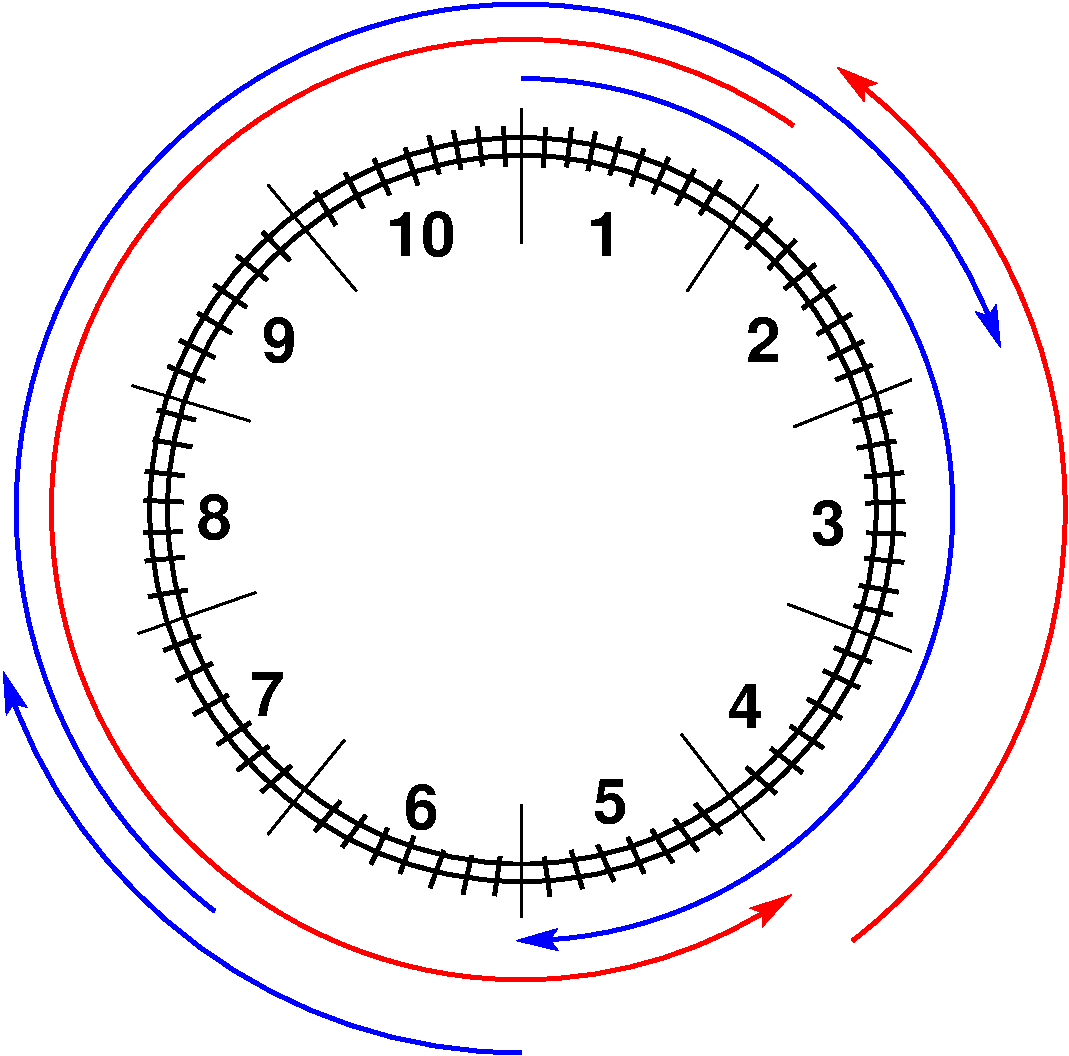
\includegraphics[width=0.5\textwidth]{alternatingfig.pdf}
\end{center}
\vspace{1mm}

{\em Eine Lösung des ersten Beispiels. Die gebogenen Pfeile um die Schienen representieren die Drähte, die den Strom liefern. Die Richtung jedes Pfeiles repräsentiert Fredriks Wahl der Richtung des Stromes (wobei die blauen und roten Farben die unterschiedliche Richtungen betonen). Beachte, dass alle Pfeile invertiert werden können, um eine weitere mögliche Lösung zu erzielen: \texttt{11010}.}

%{\em A solution to the first sample. The curved arrows outside the railway represent the wires that provide electricity. The direction of each arrow represents Fredrik's choice of direction of the current (with the blue and red colors emphasizing the different directions). Note that all arrows could have been reversed to get the other valid solution: \texttt{11010}.}

\section*{\inputsection}
Die erste Zeile der Eingabe enthält zwei Zahlen $N$ und $M$, die Anzahl der Schienen und die Anzahl der Drähte.

Die nächsten $M$ Zeilen enthalten jeweils zwei Zahlen $1 \le a, b \le N$, die bedeuten, dass es einen Draht gibt, der die Schienen $a, a+1, \dots, b$ verbindet. Wenn $b$ kleiner als $a$ ist, bedeutet das, dass sich der Draht über den Ursprung hinweg spannt, also über die Schienen $a, \dots, N, 1, \dots, b$. Falls $a=b$, versorgt der Draht nur eine Schiene mit Strom.


%The first line contains two integers $N$ and $M$, the number of railway segments and the number of wires, respectively.

%The next $M$ lines each contains two numbers $1 \le a, b \le N$, indicating that there is a wire that covers segments $a, a+1, \dots, b$. If $b$ is smaller than $a$, it means that the sequence wraps around, i.e. segments $a, \dots, N, 1, \dots, b$ are covered. Note that if $a=b$, the wire covers only one segment.

\section*{\outputsection}
Gib eine einzelne Zeile mit $M$ Zeichen aus, die jeweils \texttt{0} oder \texttt{1} sein dürfen. Das $i$-te Zeichen soll \texttt{0} sein, wenn der Strom im $i$-ten Draht der Eingabe im Uhrzeigersinn ausgerichtet sein soll, und \texttt{1}, wenn der Strom gegen den Uhrzeigersinn ausgerichtet sein soll. Wenn es mehrere Lösungen gibt, gib eine beliebige davon aus.

Wenn es keine Lösung gibt, gib ``\texttt{impossible}'' aus.

%Output a single line with $M$ characters, each being either \texttt{0} or \texttt{1}. The $i$th character of the line should be \texttt{0} if the current in the $i$th wire given in the input should be  directed clockwise, or \texttt{1} if it should be directed counter-clockwise. If there are multiple solutions you may output any of them.

%If there is no valid solution, output ``\texttt{impossible}''.

\section*{\constraints}
\testgroups

\noindent
\begin{tabular}{| l | l | l | l |}
\hline
\textbf{\group} & \textbf{\points} & \textbf{\limitsname} & \textbf{\additionalconstraints} \\ \hline
  1     & 13     & $2 \le N, M \le 15$ & \\ \hline
  2     & 20     & $2 \le N, M \le 100$ & \\ \hline
  3     & 22     & $2 \le N, M \le 1000$ & \\ \hline
  4     & 19     & $2 \le N, M \le 100\,000$ & Für keinen Draht gilt $b < a$. \\ \hline
  5     & 26     & $2 \le N, M \le 100\,000$ & \\ \hline
\end{tabular}

